
\begin{frame}
 \frametitle{Demo 8-1 $\vert$ \bfseries Isotropy}
 \framesubtitle{\bfseries tension test}
  \begin{overlayarea}{0.9\textwidth}{0.9\textheight}

 \begin{center}
 \begin{tikzpicture}[scale=3]
  \fill[gray!10, draw=black] (0, 1) rectangle (1, 0) node[above left, black]{$\mathcal{B}$};

  \draw[thin,gray] (0, 1) -- +(0, 0.2);
  \draw[thin,gray] (1, 1) -- +(0, 0.2);
  \draw[<->,thin,gray] (0, 1.15) -- node[fill=white]{$\ell$} +(1, 0);
  \draw[thin,gray] (1, 0) -- +(0.6, 0);
  \draw[thin,gray] (1, 1) -- +(0.6, -0);
  \draw[<->,gray] (1.55, 0) -- node[fill=white,sloped]{$\ell$} +(0, 1);

   \draw[thick,-latex] (0, 0) -- +(0.5, 0) node[above]{$\v e_1$};
   \draw[thick,-latex] (0, 0) -- +(0, 0.5) node[right]{$\v e_2$};

  \foreach \x in {0.0,0.1666,0.333,...,1.0}
  \draw[thick,-latex] (1, 0.05+0.9/1.0*\x) -- +(0.2, 0);
  \node at (1.2, 0.8) [right,xshift=0.0cm]{$\v u^p$};

  \fill[pattern=north west lines, pattern color=black] (-0.1, -0.05) rectangle +(-0.1, 1.1);
  \draw[thick] (-0.1, -0.05) -- +(0, 1.1);
  \draw[yshift=0.05cm] (0, 0) -- +(-0.07, 0.06) -- +(-0.07, -0.06) -- (0,0) +(-0.07, -0.1) -- +(-0.07, 0.1);
  \draw[yshift=0.95cm] (0, 0) -- +(-0.07, 0.06) -- +(-0.07, -0.06) -- (0,0) +(-0.07, -0.1) -- +(-0.07, 0.1);

  \fill[pattern=north west lines, pattern color=black] (-0.05, -0.1) rectangle +(1.1, -0.1);
  \draw[thick] (-0.05, -0.1) -- +(1.1, 0);
  \draw[xshift=0.05cm,rotate=90] (0, 0) -- +(-0.07, 0.06) -- +(-0.07, -0.06) -- (0,0) +(-0.07, -0.1) -- +(-0.07, 0.1);
  \draw[xshift=0.95cm,rotate=90] (0, 0) -- +(-0.07, 0.06) -- +(-0.07, -0.06) -- (0,0) +(-0.07, -0.1) -- +(-0.07, 0.1);

%   \fill[pattern=north west lines, pattern color=black] (3, -0.25) rectangle +(0.25, 1.5);
%   \draw[thick] (3, -0.25) -- +(0, 1.5);
  
  \begin{scope}
   \onslide<1>{\node at (-0.2, -0.7) [right]{\parbox{4cm}{\begin{align*} E &= 200 \, \mathrm{GPa} \\ \nu &= 0.5, \, 0.3, \, 0.0, \, -0.5 \\ \ell &= 1\,\mathrm{m} \end{align*}}};}
   \onslide<1>{\node at (1.7, -0.7) [right]{$[u^p_i] = \begin{bmatrix} 0.2 \ell \\ 0 \\ 0 \end{bmatrix}$};}
  \end{scope}
  
  \end{tikzpicture}
  \end{center}

 \end{overlayarea}
\end{frame}



\begin{frame}
 \frametitle{Demo 8-1 $\vert$ \bfseries Isotropy}
 \framesubtitle{\bfseries tension test}
  \vspace*{-2ex}
  \hspace*{-2em}
  \begin{tikzpicture}
  \node at(0,0) {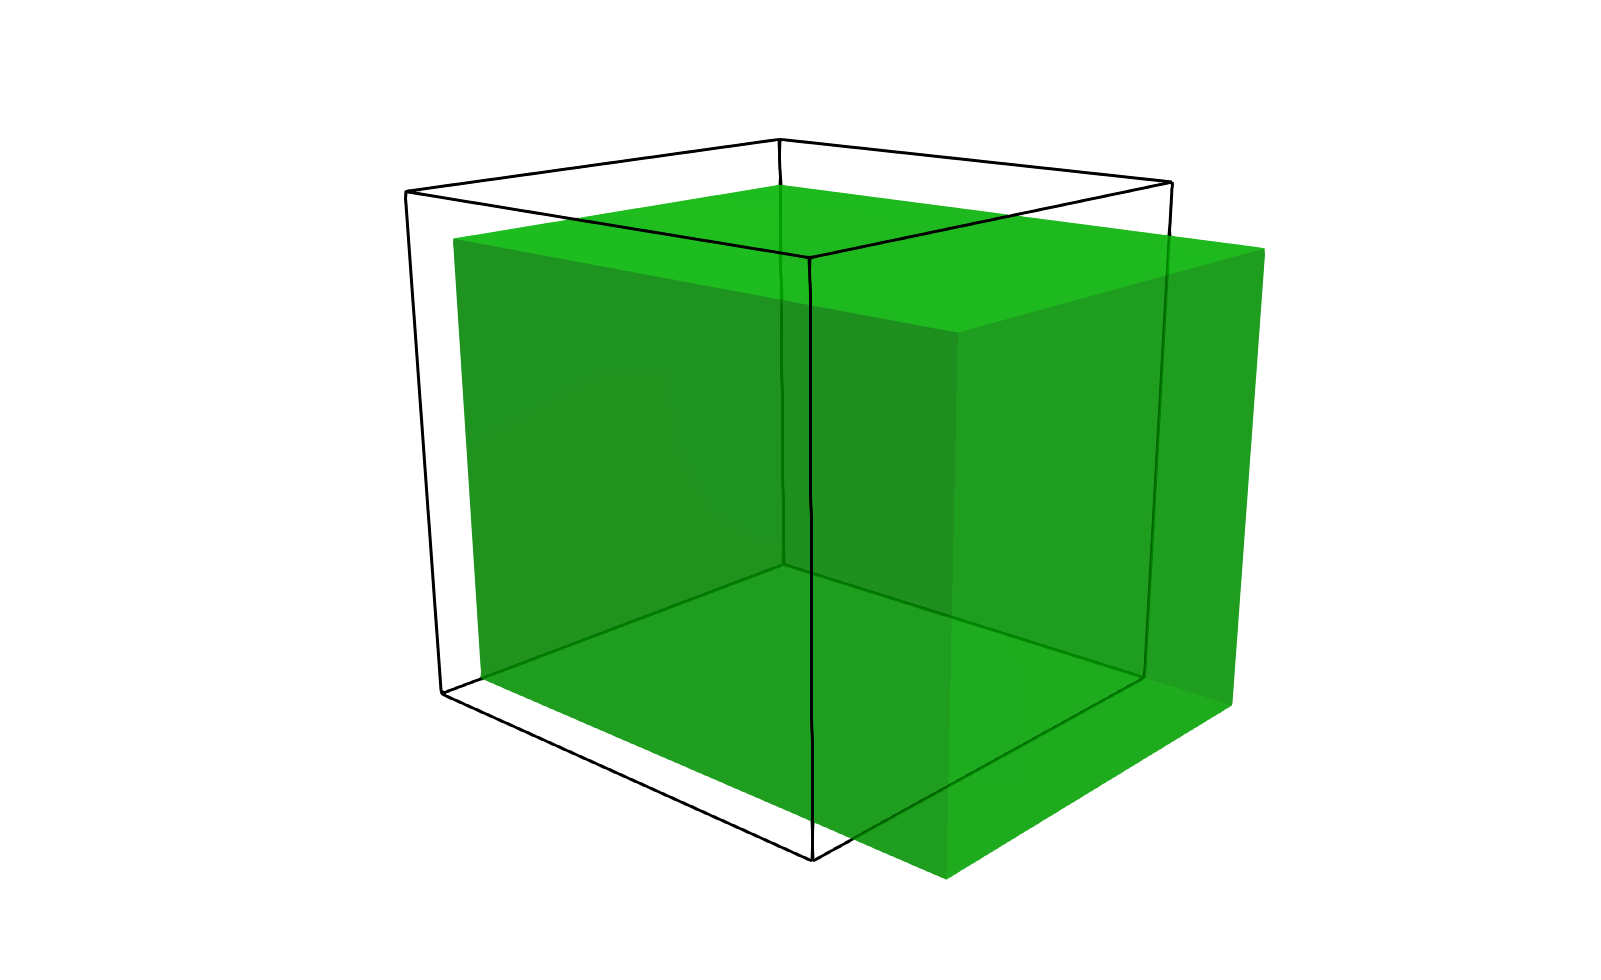
\includegraphics[width=6cm]{../08-isotropy/01-tension/tension_05.png}};
  \node at(6,0) {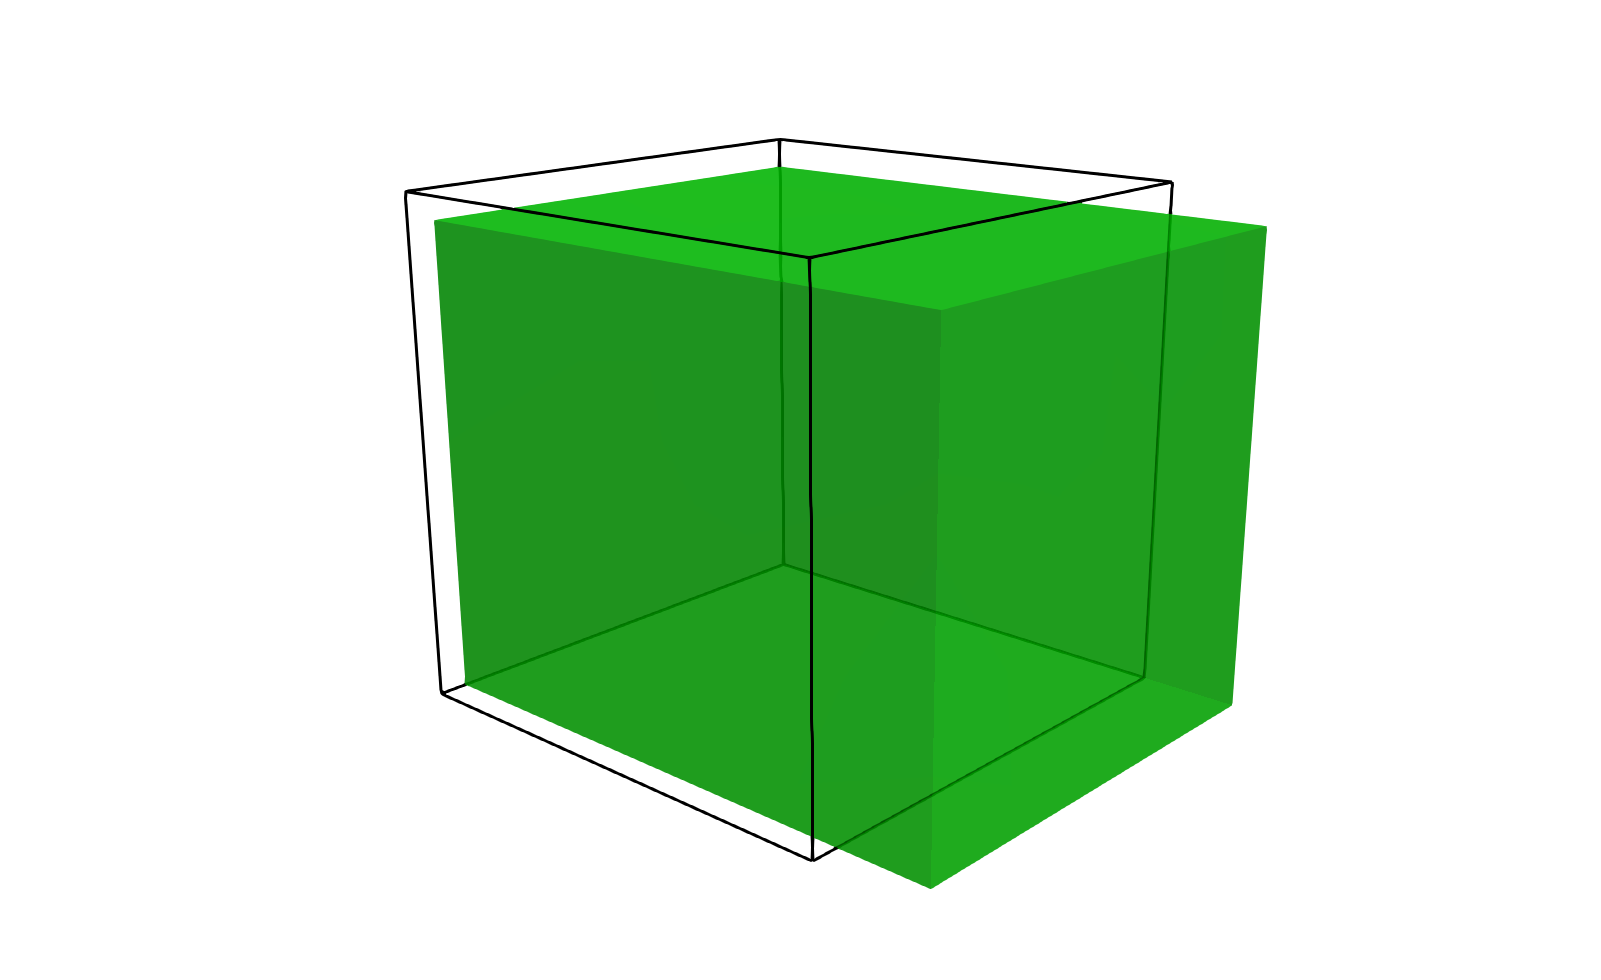
\includegraphics[width=6cm]{../08-isotropy/01-tension/tension_03.png}};
  \node at(0,-4) {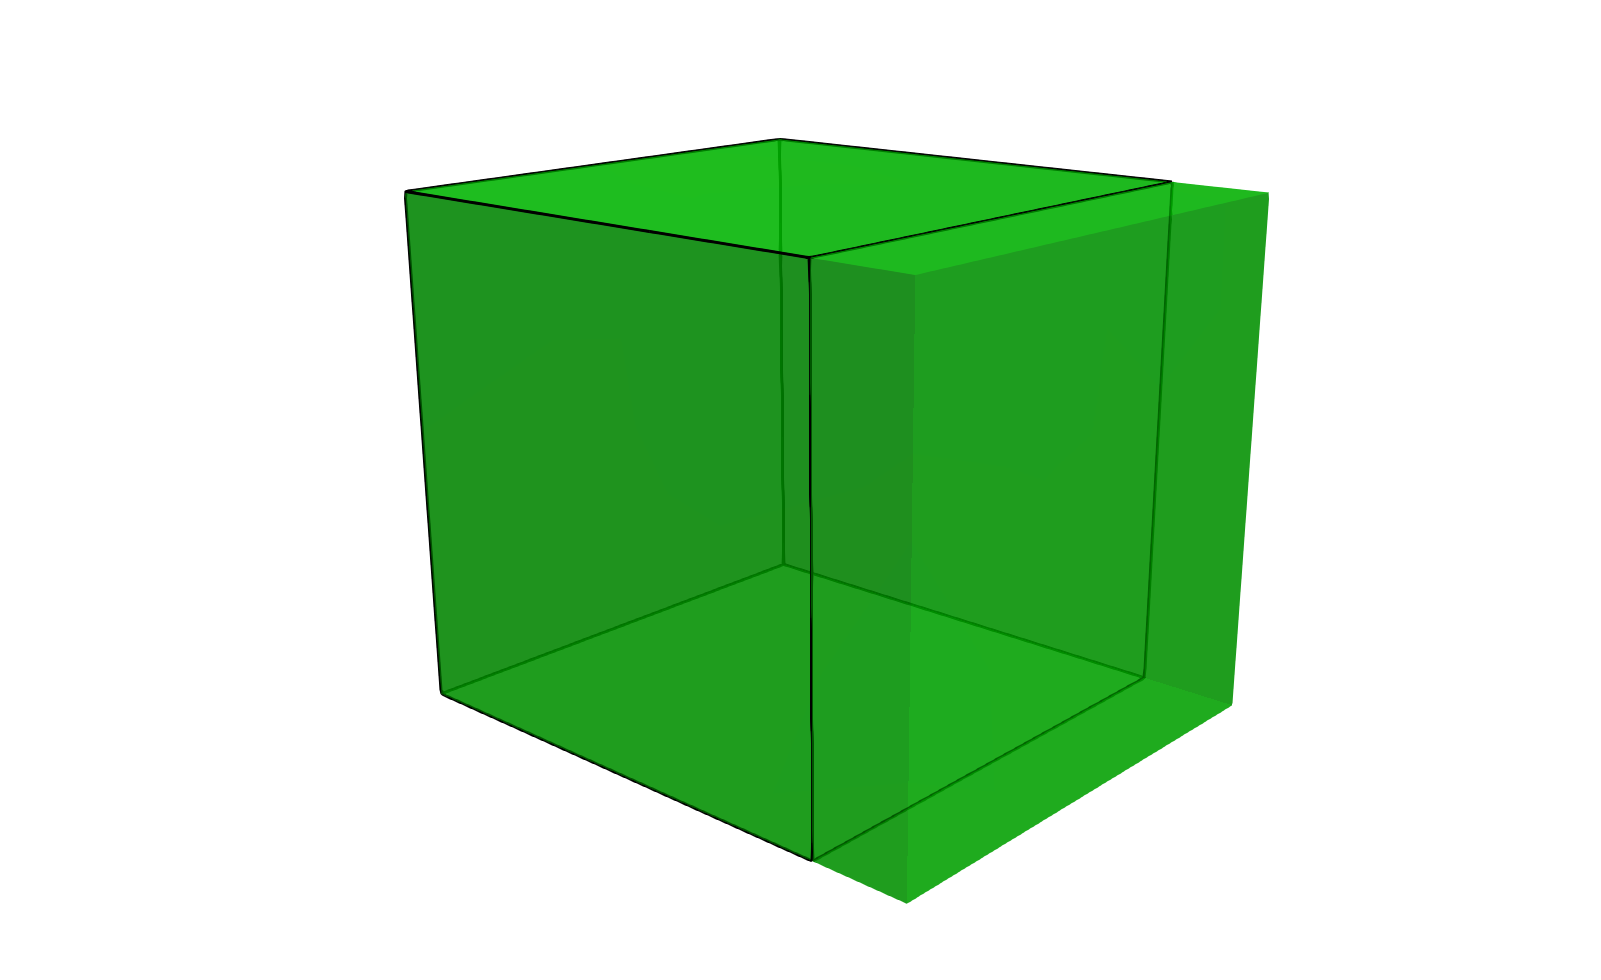
\includegraphics[width=6cm]{../08-isotropy/01-tension/tension_00.png}};
  \node at(6,-4) {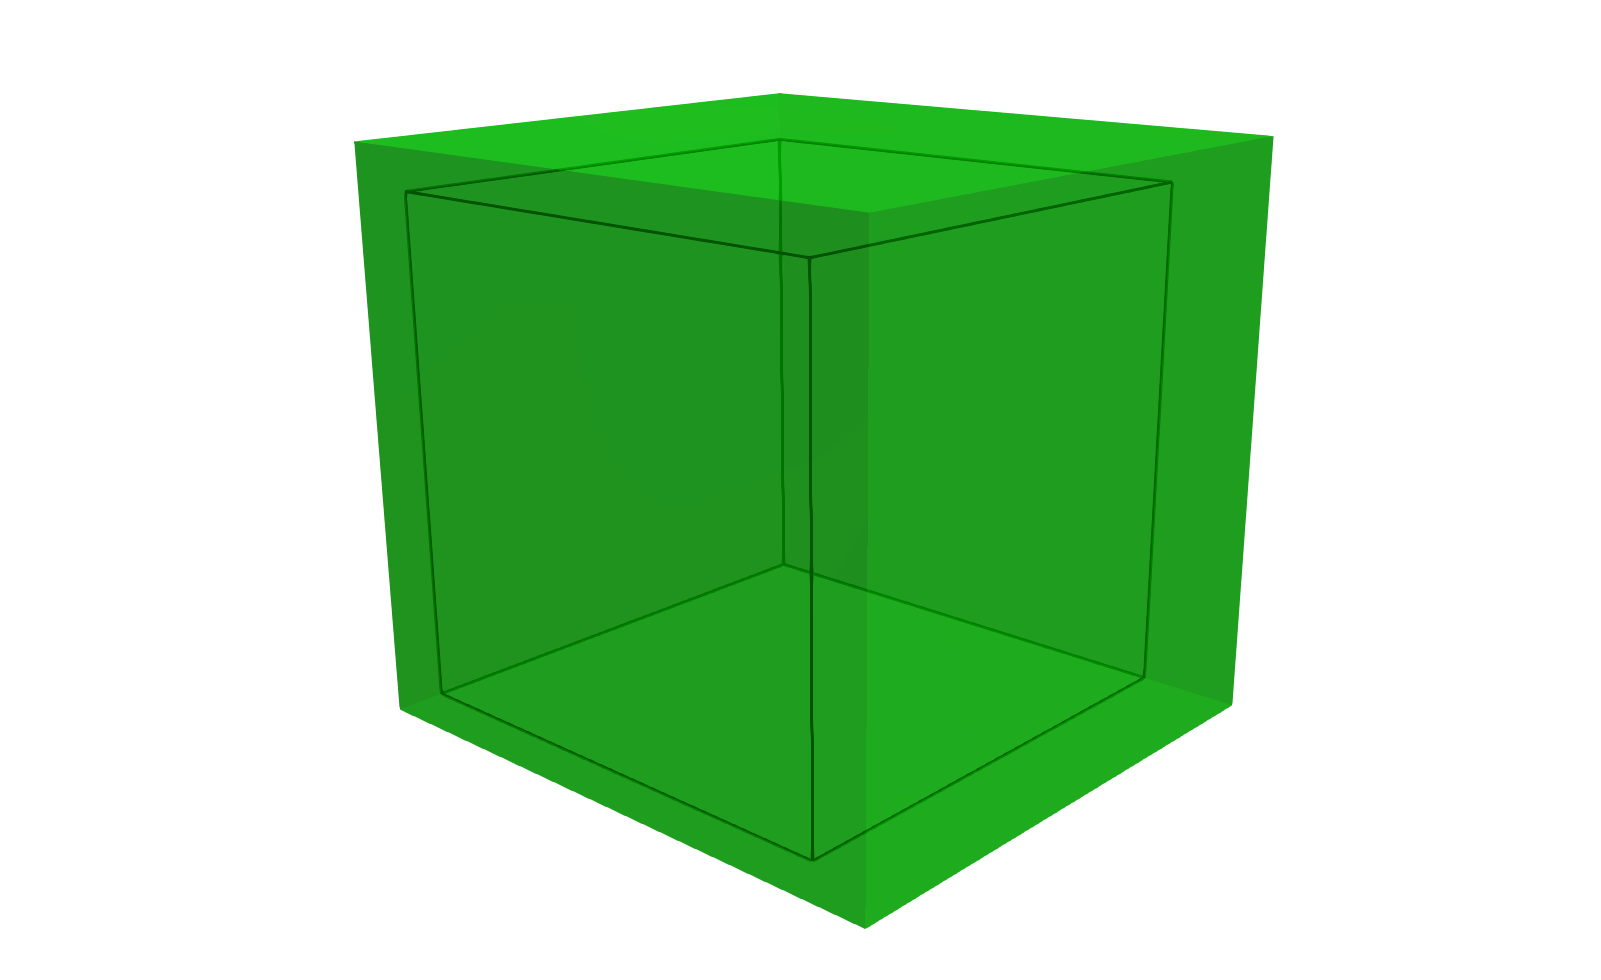
\includegraphics[width=6cm]{../08-isotropy/01-tension/tension_-05.png}};
  
  \node at(-2.5, 0) {\parbox{2cm}{\begin{align*} \nu &= 0.5 \end{align*}}};
  \node at(-2.5, -0.5) [font=\scriptsize]{(incompressible)};
  \node at(3.5, 0) {\parbox{2cm}{\begin{align*} \nu &= 0.3 \end{align*}}};
  \node at(-2.5, -4) {\parbox{2cm}{\begin{align*} \nu &= 0.0 \end{align*}}};
  \node at(3.5, -4) {\parbox{2cm}{\begin{align*} \nu &= -0.5 \end{align*}}};
  \node at(3.5, -4.5) [font=\scriptsize]{(auxetic)};
  \end{tikzpicture}
\end{frame}



\begin{frame}
 \frametitle{Demo 8-2 $\vert$ \bfseries Isotropy}
 \framesubtitle{\bfseries compression test}
  \begin{overlayarea}{0.9\textwidth}{0.9\textheight}
  \vspace*{-3ex}
 \begin{center}
 \begin{tikzpicture}[scale=3]
  \fill[gray!10, draw=black] (0, 1) rectangle (1, 0) node[above left, black]{$\mathcal{B}$};

  \draw[thin,gray] (0, 1) -- +(0, 0.4);
  \draw[thin,gray] (1, 1) -- +(0, 0.4);
  \draw[<->,thin,gray] (0, 1.35) -- node[fill=white]{$\ell$} +(1, 0);
  \draw[thin,gray] (1, 0) -- +(0.6, 0);
  \draw[thin,gray] (1, 1) -- +(0.6, -0);
  \draw[<->,gray] (1.55, 0) -- node[fill=white,sloped]{$\ell$} +(0, 1);

   \draw[thick,-latex] (0, 0) -- +(0.5, 0) node[above]{$\v e_1$};
   \draw[thick,-latex] (0, 0) -- +(0, 0.5) node[right]{$\v e_2$};

   \foreach \x in {0.0,0.1666,0.333,...,1.0} {
    \draw[-latex] (1.2, 0.05+0.9/1.0*\x) -- +(-0.2, 0);
    \draw[-latex] (0.05+0.9/1.0*\x, 1.2) -- +(0, -0.2);
  }
  \draw (0.05, 1.2) -- +(0.9, 0);
  \draw (1.2, 0.05) -- +(0, 0.9);
  \node at (1.2, 0.8) [right,xshift=0.0cm]{$\v t^p$};
  
%   \foreach \x in {0.0,0.1666,0.333,...,1.0}
%   \draw[thick,-latex] (1, 0.05+0.9/1.0*\x) -- +(0.2, 0);
%   \node at (1.2, 0.8) [right,xshift=0.0cm]{$\v u^p$};

  \fill[pattern=north west lines, pattern color=black] (-0.1, -0.05) rectangle +(-0.1, 1.1);
  \draw[thick] (-0.1, -0.05) -- +(0, 1.1);
  \draw[yshift=0.05cm] (0, 0) -- +(-0.07, 0.06) -- +(-0.07, -0.06) -- (0,0) +(-0.07, -0.1) -- +(-0.07, 0.1);
  \draw[yshift=0.95cm] (0, 0) -- +(-0.07, 0.06) -- +(-0.07, -0.06) -- (0,0) +(-0.07, -0.1) -- +(-0.07, 0.1);

  \fill[pattern=north west lines, pattern color=black] (-0.05, -0.1) rectangle +(1.1, -0.1);
  \draw[thick] (-0.05, -0.1) -- +(1.1, 0);
  \draw[xshift=0.05cm,rotate=90] (0, 0) -- +(-0.07, 0.06) -- +(-0.07, -0.06) -- (0,0) +(-0.07, -0.1) -- +(-0.07, 0.1);
  \draw[xshift=0.95cm,rotate=90] (0, 0) -- +(-0.07, 0.06) -- +(-0.07, -0.06) -- (0,0) +(-0.07, -0.1) -- +(-0.07, 0.1);

%   \fill[pattern=north west lines, pattern color=black] (3, -0.25) rectangle +(0.25, 1.5);
%   \draw[thick] (3, -0.25) -- +(0, 1.5);
  
  \begin{scope}
   \onslide<1>{\node at (-0.2, -0.7) [right]{\parbox{4cm}{\begin{align*} E &= 200 \, \mathrm{GPa} \\ \nu &= 0.5, \, 0.3, \, 0.0, \, -0.5 \\ \ell &= 1\,\mathrm{m} \end{align*}}};}
%    \onslide<1>{\node at (1.5, -0.7) [right]{$[u^p_i] = -\begin{bmatrix} 0.2 \ell \\ 0 \\ 0 \end{bmatrix}$ on $\partial \mathcal{B}^t_\text{right}$};}
   \onslide<1>{\node at (1.7, -0.7) [right]{$\vert \v t^p \vert = 50 \, \mathrm{MPa}$};}
  \end{scope}
  
  \end{tikzpicture}
  \end{center}

 \end{overlayarea}
\end{frame}


\begin{frame}
 \frametitle{Demo 8-2 $\vert$ \bfseries Isotropy}
 \framesubtitle{\bfseries compression test}
  \vspace*{-2ex}
  \hspace*{-2em}
  \begin{tikzpicture}
  \node at(0,0) {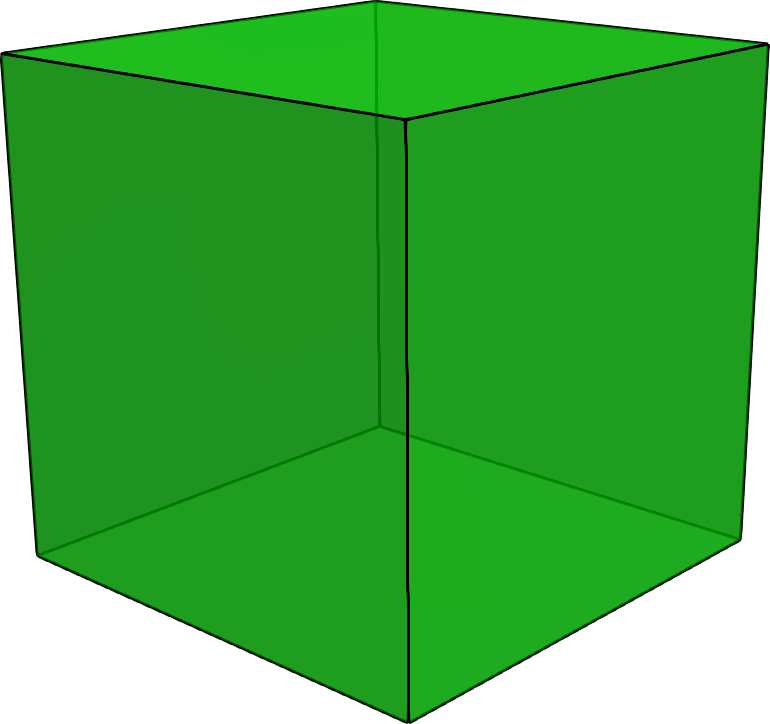
\includegraphics[width=3cm]{../08-isotropy/02-compression/comp_05.png}};
  \node at(6,0) {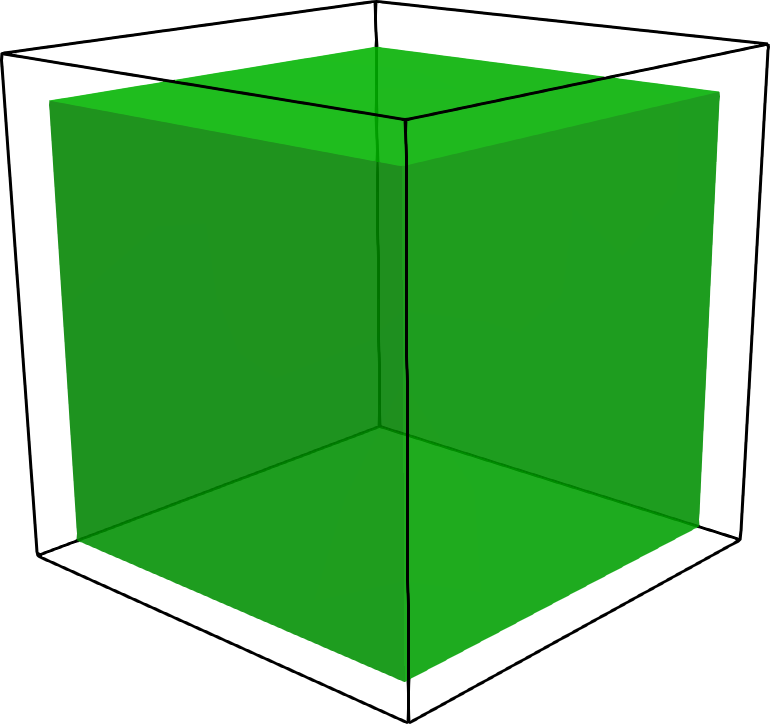
\includegraphics[width=3cm]{../08-isotropy/02-compression/comp_03.png}};
  \node at(0,-3.8) {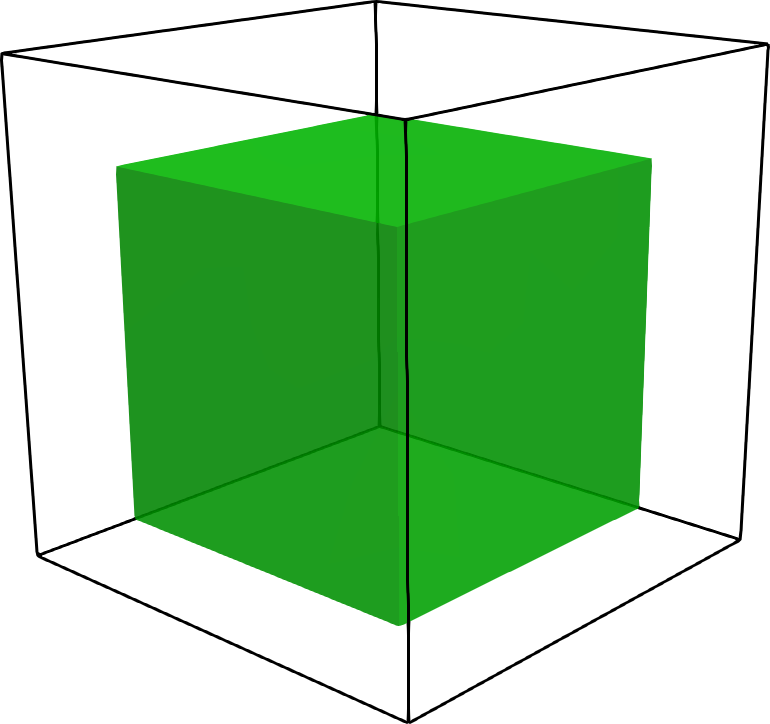
\includegraphics[width=3cm]{../08-isotropy/02-compression/comp_00.png}};
  \node at(6,-3.8) {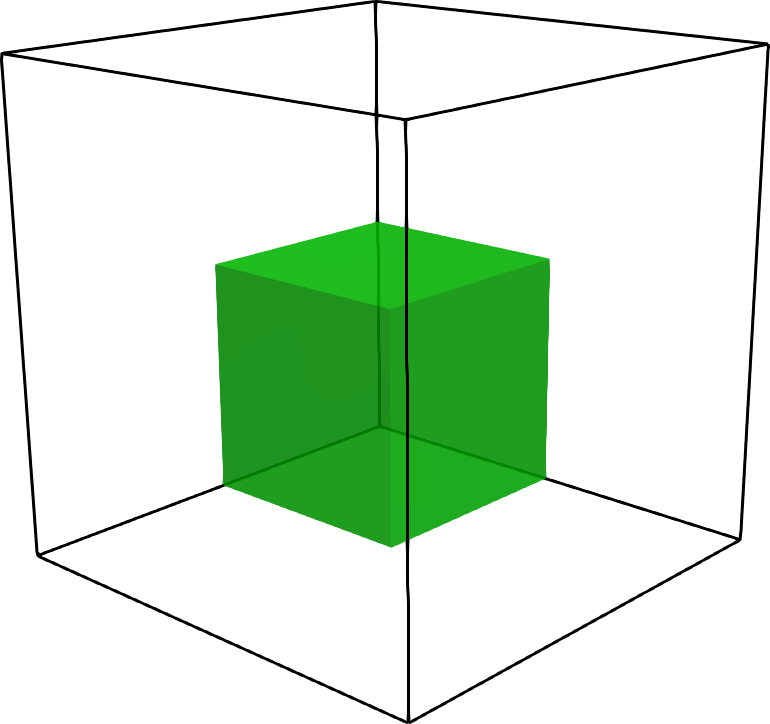
\includegraphics[width=3cm]{../08-isotropy/02-compression/comp_-05.png}};
  
  \node at(-2.6, -0.7) {\parbox{2cm}{\begin{align*} \nu &= 0.5 \\[-0.5ex] \rightarrow K &= \infty \end{align*}}};
  \node at(-2.4, -1.5) [font=\scriptsize]{(incompressible)};
  \node at(3.4, -0.7) {\parbox{2cm}{\begin{align*} \nu &= 0.3 \\[-0.5ex] \rightarrow K &\approx 167\,\mathrm{GPa} \end{align*}}};
  \node at(-2.6, -4.5) {\parbox{2cm}{\begin{align*} \nu &= 0.0 \\[-0.5ex] \rightarrow K &\approx 67\,\mathrm{GPa} \end{align*}}};
  \node at(3.4, -4.5) {\parbox{2cm}{\begin{align*} \nu &= -0.5 \\[-0.5ex] \rightarrow K &\approx 33\,\mathrm{GPa} \end{align*}}};
  \node at(3.4, -5.3) [font=\scriptsize]{(auxetic)};
  
  \node at (0, -6) [right,font=\footnotesize]{$\v u$ scaled with a factor of $1000$};
  \end{tikzpicture}
\end{frame}

